\documentclass{../notes}

\title{Arbres et graphes}

\newlength\stextwidth
\newcommand\makesamewidth[3][c]{%
  \settowidth{\stextwidth}{#2}%
  \makebox[\stextwidth][#1]{#3}%
}

\newcounter{questioncounter}
\setcounter{questioncounter}{0}

\newcommand\question[1]{
  \vspace{1em}
  \refstepcounter{questioncounter}
  \makesamewidth[r]{\textbf{Q99.}}{\textbf{Q\thequestioncounter.}}~
  \parbox[t]{11cm}{#1}
  \vspace{1em}
}

\newcommand\monoit[1]{ \texttt{\textit{#1}} }

\newcommand\indication[2]{
  \textit{Indication #1.}

  \raisebox{\depth}{\rotatebox{180}{\parbox{12.3cm}{#2}}}
}

\usepackage{leftindex}

\begin{document}
  \tableofcontents
  \clearpage

  \section{Décomposition en composantes connexes}

  \subsection{Graphe non-orienté}

  Considérons un graphe non-orienté $G = (V, E)$.
  Ce graphe n'est pas nécessairement connexe, mais on peut le décomposer en différentes composantes avec chacune des composante connexe.

  \begin{defn}
    Une partie $X \subseteq V$ d'un graphe $G = (V, E)$ est dite \textit{connexe}, si pour tous $x, y \in X$, avec $x \neq y$, il existe $v_1, \ldots, v_n \in X$ (pour un certain $n$) tel que \[
    x - v_1 - v_2 - \cdots - v_{n-1} - v_n - y
    ,\]
    où l'on note $a - b$ lorsque $\{a,b\} \in E$.

    On dit qu'un graphe $G = (V, E)$ est \textit{connexe} si $V$ est connexe.
    \label{defn-connexe}
  \end{defn}

  On notera $a -^\star b$ lorsqu'il existe un chemin (possiblement vide dans le cas $a = b$) de $a$ vers $b$.

  \question{Montrer que $-^\star$ est une relation d'équivalence sur~$V$.}

  \question{Reformuler la définition~\ref{defn-connexe} en terme de classe d'équivalence de~$-^\star$.}

  La décomposition de $G$ en composantes connexes est possible car les classes d'équivalences de $-^\star$ forment un partitionnement de $V$.
  La question est maintenant de déterminer ce partitionnement.

  \begin{figure}[H]
    \centering
    \begin{tikzpicture}[node distance=180]
      \begin{scope}[name=G1, node distance=60, local bounding box=G1b]
        \node[fill, scale=0.5, circle]             (a) {};
        \node[fill, scale=0.5, circle, below of=a] (b) {};
        \node[fill, scale=0.5, circle, right of=a] (c) {};
        \node[fill, scale=0.5, circle, right of=b] (d) {};
        \node[fill, scale=0.5, circle, right of=c] (e) {};
        \node[fill, scale=0.5, circle, right of=d] (f) {};
        \draw (a) -- (b) -- (c);
        \draw (e) -- (f);
      \end{scope}
      \begin{scope}[name=G2, right of=G1, node distance=60, local bounding box=G2b]
        \node[fill, scale=0.5, circle]             (a) {};
        \node[fill, scale=0.5, circle, below of=a] (b) {};
        \node[fill, scale=0.5, circle, right of=a] (c) {};
        \node[fill, scale=0.5, circle, right of=b] (d) {};
        \node[fill, scale=0.5, circle, right of=c] (e) {};
        \node[fill, scale=0.5, circle, right of=d] (f) {};
        \draw (a) -- (b) -- (c);
        \draw (e) -- (f);
        \begin{pgfonlayer}{background}
          \filldraw[line width=15pt, line cap=round, line join=round, nicered] (e.center) -- (f.center);
          \filldraw[line width=15pt, line cap=round, line join=round, nicered] (d.center) -- (d.center);
          \filldraw[line width=15pt, line cap=round, line join=round, nicered] (a.center) -- (b.center) -- (c.center) -- cycle;
        \end{pgfonlayer}
      \end{scope}
      \tikzset{node distance=50};
      \node[right of=G1b] (X) {};
      \node[left of=G2b] (Y) {};
      \draw[->] (X) to node[midway,below] {comp. connexes} (Y);
    \end{tikzpicture}
    \caption{Composantes connexes dans un graphe}
  \end{figure}

  \question{Comment peut-on calculer simplement la composante connexe contenant un sommet $v \in V$ fixé ?}

  \question{En déduire une méthode pour calculer le partitionnement en composantes connexes.\label{Q-partitionnement-no}}

  \subsection{Graphe orienté -- algorithme de Kosaraju}

  Considérons un graphe $G = (V, E)$ orienté.

  \begin{defn}
    Une partie $X \subseteq V$ est \textit{fortement connexe} si, pour tout $x,y \in V$ avec $x \neq y$, il existe $u_1, \ldots, u_n$ et $v_1, \ldots, v_m$ (pour un certain couple $(n, m)$) tels que 
    \[
    \begin{tikzcd}[row sep=5, column sep=10]
      & u_1 \arrow{r}{} & u_2 \arrow{r}{} & \cdots \arrow{r}{} & u_n \arrow{dr}{}\\
      x \arrow{ur}{} & & & & & y \arrow{dl}{} \\
      & v_m \arrow{ul}{} & \cdots \arrow{l}{} & v_2 \arrow{l}{} & v_1 \arrow{l}
    \end{tikzcd}
    .\]
  \end{defn}
  On note alors $x \overset \star \rightleftarrows y$ lorsqu'il existe un chemin de $x$ à $y$ (noté $x \to^\star y$) et un chemin de $y$ à $x$ (noté $x \leftindex^\star{\gets} y$).
  Ces deux chemins peuvent être distincts.

   \begin{figure}[H]
     \centering
     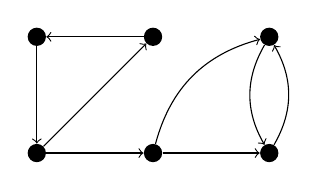
\begin{tikzpicture}[node distance=60]
      \node[fill, scale=0.7, circle]             (a) {};
      \node[fill, scale=0.7, circle, below of=a] (b) {};
      \node[fill, scale=0.7, circle, right of=a] (c) {};
      \node[fill, scale=0.7, circle, right of=b] (d) {};
      \node[fill, scale=0.7, circle, right of=c] (e) {};
      \node[fill, scale=0.7, circle, right of=d] (f) {};
      \draw[->] (a) to (b);
      \draw[->] (b) to (c);
      \draw[->] (c) to (a);
      \draw[->] (b) to (d);
      \draw[->] (d) to[bend left] (e);
      \draw[->] (d) to (f);
      \draw[->] (e) to[bend right] (f);
      \draw[->] (f) to[bend right] (e);
     \end{tikzpicture}
     \caption{Un graphe orienté}
     \label{fig:oriented-example}
  \end{figure}

  \question{Justifier brièvement que $\overset \star \rightleftarrows$ est une relation d'équivalence sur~$V$. Que sont les classes d'équivalences de cette relation ?}

  \question{En appliquant la méthode utilisée en question~\ref{Q-partitionnement-no} au graphe en figure~\ref{fig:oriented-example}, que donne le partitionnement ?}

  Dommage, on n'a pas les composantes fortement connexes.
  Il faut travailler un peu plus pour les trouver\ldots

  Un parcours d'un graphe (en largeur, en profondeur, peu importe) induit une forêt, c'est-à-dire un graphe non-orienté dont les composantes connexes sont des arbres. Autrement dit, une forêt, c'est un graphe acyclique car un arbre est un graphe non-orienté acyclique et connexe.

  \begin{figure}[H]
     \centering
     \begin{tikzpicture}[node distance=60]
      \node[fill, scale=0.7, circle]             (a) {};
      \node[fill, scale=0.7, circle, below of=a] (b) {};
      \node[fill, scale=0.7, circle, right of=a] (c) {};
      \node[fill, scale=0.7, circle, right of=b] (d) {};
      \node[fill, scale=0.7, circle, right of=c] (e) {};
      \node[fill, scale=0.7, circle, right of=d] (f) {};
      \draw[->] (a) to (b);
      \draw[->] (b) to (c);
      \draw[->] (c) to (a);
      \draw[->] (b) to (d);
      \draw[->] (d) to[bend left] (e);
      \draw[->] (d) to (f);
      \draw[->] (e) to[bend right] (f);
      \draw[->] (f) to[bend right] (e);
      \tikzset{node distance=10};
      \node[below of=d, deepblue] (td) {1};
      \node[below of=f, deepblue] (tf) {2};
      \node[above of=e, deepblue] (te) {3};
      \node[above of=a, deepblue] (ta) {4};
      \node[below of=b, deepblue] (tb) {5};
      \node[above of=c, deepblue] (tc) {6};
      \begin{pgfonlayer}{background}
        \node[fit=(a)(ta), rectangle, fill=deepblue, nearly transparent] (ba) {};
        \node[fit=(b)(tb), rectangle, fill=deepblue, nearly transparent] (bb) {};
        \node[fit=(c)(tc), rectangle, fill=deepblue, nearly transparent] (bc) {};
        \node[fit=(d)(td), rectangle, fill=deepblue, nearly transparent] (bd) {};
        \node[fit=(e)(te), rectangle, fill=deepblue, nearly transparent] (be) {};
        \node[fit=(f)(tf), rectangle, fill=deepblue, nearly transparent] (bf) {};
      \end{pgfonlayer}
      \draw[very thick, deepblue, -latex] (f) to (e);
      \draw[very thick, deepblue, -latex] (d) to (f);
      \draw[very thick, deepblue, -latex] (a) to (b);
      \draw[very thick, deepblue, -latex] (b) to (c);
     \end{tikzpicture}
     \hspace{4em}
     \begin{tikzpicture}[node distance=60]
      \node[fill, scale=0.7, circle]             (a) {};
      \node[fill, scale=0.7, circle, below of=a] (b) {};
      \node[fill, scale=0.7, circle, right of=a] (c) {};
      \node[fill, scale=0.7, circle, right of=b] (d) {};
      \node[fill, scale=0.7, circle, right of=c] (e) {};
      \node[fill, scale=0.7, circle, right of=d] (f) {};
      \draw[->] (a) to (b);
      \draw[->] (b) to (c);
      \draw[->] (c) to (a);
      \draw[->] (b) to (d);
      \draw[->] (d) to[bend left] (e);
      \draw[->] (d) to (f);
      \draw[->] (e) to[bend right] (f);
      \draw[->] (f) to[bend right] (e);
      \tikzset{node distance=10};
      \node[above of=a, deepblue] (ta) {1};
      \node[below of=b, deepblue] (tb) {2};
      \node[above of=c, deepblue] (tc) {3};
      \node[below of=d, deepblue] (td) {4};
      \node[above of=e, deepblue] (te) {5};
      \node[below of=f, deepblue] (tf) {6};
      \begin{pgfonlayer}{background}
        \node[fit=(a)(ta), rectangle, fill=deepblue, nearly transparent] (ba) {};
        \node[fit=(b)(tb), rectangle, fill=deepblue, nearly transparent] (bb) {};
        \node[fit=(c)(tc), rectangle, fill=deepblue, nearly transparent] (bc) {};
        \node[fit=(d)(td), rectangle, fill=deepblue, nearly transparent] (bd) {};
        \node[fit=(e)(te), rectangle, fill=deepblue, nearly transparent] (be) {};
        \node[fit=(f)(tf), rectangle, fill=deepblue, nearly transparent] (bf) {};
      \end{pgfonlayer}
      \draw[very thick, deepblue, -latex] (a) to (b);
      \draw[very thick, deepblue, -latex] (b) to (c);
      \draw[very thick, deepblue, -latex] (b) to (d);
      \draw[very thick, deepblue, -latex] (d) to (e);
      \draw[very thick, deepblue, -latex] (d) to (f);
     \end{tikzpicture}
     \caption{Deux forêts de parcours}
     \label{fig:foret-parcours}
  \end{figure}

  Avant de passer à l'algorithme pour décomposer $G$ en composantes fortement connexes, on doit réaliser un \textit{parcours en profondeur daté}.

  Lors d'un parcours en profondeur, on a deux cas :
  \begin{itemize}
    \item soit on continue d'explorer le sous-arbre, et dans ce cas, on ne fait rien de plus ;
    \item soit on passe à un nouveau sous-arbre (s'applique aussi si l'on n'a rien exploré avant), et dans ce cas, on note la "date de fin" pour l'ancien sous-arbre, et on note la "date de début" pour le sous-arbre suivant.
  \end{itemize}
  Dans la figure~\ref{fig:foret-parcours}, on n'a noté que les dates de débuts.
  On rajoute les dates de fin, comme montré dans la figure~\ref{fig:foret-parcours-date}.
  On note "date de début"/"date de fin".

  \begin{figure}[H]
    \centering
     \begin{tikzpicture}[node distance=80]
      \node[fill, scale=0.7, circle]             (a) {};
      \node[fill, scale=0.7, circle, below of=a] (b) {};
      \node[fill, scale=0.7, circle, right of=a] (c) {};
      \node[fill, scale=0.7, circle, right of=b] (d) {};
      \node[fill, scale=0.7, circle, right of=c] (e) {};
      \node[fill, scale=0.7, circle, right of=d] (f) {};
      \draw[->] (a) to (b);
      \draw[->] (b) to (c);
      \draw[->] (c) to (a);
      \draw[->] (b) to (d);
      \draw[->] (d) to[bend left] (e);
      \draw[->] (d) to (f);
      \draw[->] (e) to[bend right] (f);
      \draw[->] (f) to[bend right] (e);
      \tikzset{node distance=10};
      \node[above of=a, deepblue, minimum width=3em] (ta) {1/12};
      \node[below of=b, deepblue, minimum width=3em] (tb) {2/11};
      \node[above of=c, deepblue, minimum width=3em] (tc) {3/4};
      \node[below of=d, deepblue, minimum width=3em] (td) {5/10};
      \node[above of=e, deepblue, minimum width=3em] (te) {6/7};
      \node[below of=f, deepblue, minimum width=3em] (tf) {8/9};
      \begin{pgfonlayer}{background}
        \node[fit=(a)(ta), rectangle, fill=deepblue, nearly transparent] (ba) {};
        \node[fit=(b)(tb), rectangle, fill=deepblue, nearly transparent] (bb) {};
        \node[fit=(c)(tc), rectangle, fill=deepblue, nearly transparent] (bc) {};
        \node[fit=(d)(td), rectangle, fill=deepblue, nearly transparent] (bd) {};
        \node[fit=(e)(te), rectangle, fill=deepblue, nearly transparent] (be) {};
        \node[fit=(f)(tf), rectangle, fill=deepblue, nearly transparent] (bf) {};
      \end{pgfonlayer}
      \draw[very thick, deepblue, -latex] (a) to (b);
      \draw[very thick, deepblue, -latex] (b) to (c);
      \draw[very thick, deepblue, -latex] (b) to (d);
      \draw[very thick, deepblue, -latex] (d) to (e);
      \draw[very thick, deepblue, -latex] (d) to (f);
     \end{tikzpicture}
    \caption{Parcours en profondeur daté}
    \label{fig:foret-parcours-date}
  \end{figure}

  Concrètement, les dates de début ne nous intéressent pas.
  Par contre, à l'aide des dates de fin (en les regardant dans l'ordre décroissant), on peut obtenir un ordre de parcours des sommets qui nous sera très utile.

  On notera $\mathrm{fin}(x)$ la date de fin d'un sommet $x$ à partir d'un parcours en profondeur daté.

  \begin{defn}
    Étant donné $G = (V, E)$, le  \textit{graphe quotient} est le graphe $\hat{G} = (\hat{V}, \hat{E})$ défini par :
    \begin{itemize}
      \item $\hat{V}$ est l'ensemble des composantes fortement connexes de $G$, \textit{i.e.} les classes d'équivalences pour $\overset \star \rightleftarrows$ ;
      \item  $\hat{E}$ est l'ensemble défini comme 
        \[
        \hat{E} = \mleft\{\, (C_1, C_2) \in \hat{V} \times \hat{V} \;\middle|\; \exists x \in C_1, \exists y \in C_2, (x,y) \in E \,\mright\} 
        .\] 
    \end{itemize}
  \end{defn}

   \begin{figure}[H]
     \centering
     \begin{tikzpicture}[node distance=60]
      \node[fill, scale=0.7, circle]             (a) {};
      \node[fill, scale=0.7, circle, below of=a] (b) {};
      \node[fill, scale=0.7, circle, right of=a] (c) {};
      \node[fill, scale=0.7, circle, right of=b] (d) {};
      \node[fill, scale=0.7, circle, right of=c] (e) {};
      \node[fill, scale=0.7, circle, right of=d] (f) {};
      \draw[->] (a) to (b);
      \draw[->] (b) to (c);
      \draw[->] (c) to (a);
      \draw[->] (b) to (d);
      \draw[->] (d) to[bend left] (e);
      \draw[->] (d) to (f);
      \draw[->] (e) to[bend right] (f);
      \draw[->] (f) to[bend right] (e);
      \begin{pgfonlayer}{background}
        \filldraw[line width=15pt, line cap=round, line join=round, nicered] (e.center) -- (f.center);
        \filldraw[line width=15pt, line cap=round, line join=round, nicered] (d.center) -- (d.center);
        \filldraw[line width=15pt, line cap=round, line join=round, nicered] (a.center) -- (b.center) -- (c.center) -- cycle;
      \end{pgfonlayer}
     \end{tikzpicture}
     \hspace{5em}
     \begin{tikzpicture}[node distance=60]
      \node[scale=0.7, circle]                   (a) {};
      \node[fill=nicered, scale=0.7, circle, below of=a] (b) {};
      \node[scale=0.7, circle, right of=a] (c) {};
      \node[fill=nicered, scale=0.7, circle, right of=b] (d) {};
      \node[scale=0.7, circle, right of=c] (e) {};
      \node[fill=nicered, scale=0.7, circle, right of=d] (f) {};
      \draw[->] (b) to (d);
      \draw[->] (d) to (f);
     \end{tikzpicture}
     \caption{Graphe quotient}
  \end{figure}

  \question{Montrer que le graphe $\hat{G}$ est acyclique (on pourra procéder par l'absurde).}

  \begin{defn}
    Un \textit{tri topologique} d'un graphe $G = (V, E)$ est une relation d'ordre totale $\preceq$ sur $V$ telle que si $x \to y$ alors $x \preceq y$.
  \end{defn}

  Dans un graphe contenant un cycle, il est impossible de trouver un tri topologique.

  \question{Trouver un ordre topologique du graphe en figure~\ref{fig:topo-exemple}.}

  \begin{figure}[H]
    \centering
    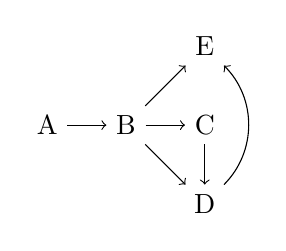
\begin{tikzpicture}
      \node (a) {A};
      \node[right of=a] (b) {B};
      \node[right of=b] (c) {C};
      \node[below of=c] (d) {D};
      \node[above of=c] (e) {E};
      \draw[->] (a) to (b);
      \draw[->] (b) to (c);
      \draw[->] (b) to (d);
      \draw[->] (c) to (d);
      \draw[->] (b) to (e);
      \draw[->] (d) to[bend right=45] (e);
    \end{tikzpicture}
    \caption{Un autre graphe (acyclique) exemple}
    \label{fig:topo-exemple}
  \end{figure}

  \question{
    On réalise un parcours en profondeur daté dans un graphe acyclique, et on construit l'ordre $\preceq$ défini par : $x \preceq y$ si et seulement si $\mathrm{fin}(x) \ge \mathrm{fin}(y)$.
    Montrer que l'on a bien construit un ordre topologique.
  }

  On définit $\mathrm{fin}(X)$ pour $X \subseteq V$ par $\mathrm{fin}(X) := \max_{x \in X} \mathrm{fin}(x)$.
  Ainsi, la date $\mathrm{fin}(X)$ correspond à la date où l'on a fini le parcours de $X$.

  \question{Démontrer que, si $C \to_{\hat{G}} C'$ alors $\mathrm{fin}(C) > \mathrm{fin}(C')$.}

  \begin{algorithm}
    \centering
    \caption{Algorithme de Kosaraju}
    \begin{algorithmic}[1]
      \State Réaliser un parcours en profondeur daté de $G$. \label{algo:kosaraju:p1}
      \State Inverser les arêtes de $G$ pour trouver $G^\intercal$  \label{algo:kosaraju:p2}
      \State Réaliser un parcours en profondeur de $G^\intercal$ en regardant les sommets de $G^\intercal$ dans l'ordre des dates de fin décroissantes. \label{algo:kosaraju:p3}
    \end{algorithmic}
    \label{algo:kosaraju}
  \end{algorithm}

  Une implémentation optimisée de l'algorithme~\ref{algo:kosaraju} peut se faire avec une complexité en $\mathrm{O}(|V| + |E|)$.
  En effet, l'étape \ref{algo:kosaraju:p1} se fait en $\mathrm{O}(|V| + |E|)$, l'étape~\ref{algo:kosaraju:p2} se fait en $\mathrm{O}(|E|)$, et l'étape~\ref{algo:kosaraju:p3} se fait en $\mathrm{O}(|V| + |E|)$.

  L'étape~\ref{algo:kosaraju:p2} n'est pas \textit{vraiment} nécessaire : il suffit, dans le parcours de l'étape~\ref{algo:kosaraju:p3}, de regarder les arêtes "à l'envers".

  \question{
    Montrer, par récurrence sur $n$, que les $n$ premiers arbres parcourus dans l'étape~\ref{algo:kosaraju:p3} sont des composantes connexes.

    Dans l'hérédité, en notant $x \in V$ le sommet utilisé pour débuter le parcours, $A_x$ l'arbre engendré par le parcours débuté à $x$, et $C_x$ la composante fortement connexe contenant $x$, on pourra montrer $A_x = C_x$ par double-inclusion.
  }

  De cela, on en déduit que l'algorithme de Kosaraju (algorithme~\ref{algo:kosaraju}) est correct.

  \question{
    Déterminer les composantes fortement connexes de l'arbre donné en figure~\ref{fig:kosaraju-application}. On utilisera exactement l'algorithme de Kosaraju, en détaillant chaque étape.
  } \label{q:kosaraju-application}

  \begin{figure}[H]
    \centering
    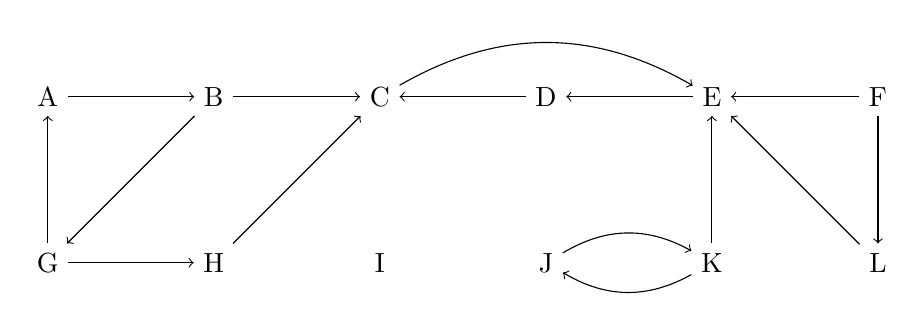
\begin{tikzpicture}[node distance=60]
      \node (a) {A};
      \node[right of=a] (b) {B};
      \node[right of=b] (c) {C};
      \node[right of=c] (d) {D};
      \node[right of=d] (e) {E};
      \node[right of=e] (f) {F};
      \node[below of=a] (g) {G};
      \node[below of=b] (h) {H};
      \node[below of=c] (i) {I};
      \node[below of=d] (j) {J};
      \node[below of=e] (k) {K};
      \node[below of=f] (l) {L};
      \draw[->] (a) to (b);
      \draw[->] (b) to (g);
      \draw[->] (g) to (a);
      \draw[->] (b) to (c);
      \draw[->] (g) to (h);
      \draw[->] (h) to (c);
      \draw[->] (d) to (c);
      \draw[->] (e) to (d);
      \draw[->] (c) to[bend left] (e);
      \draw[->] (j) to[bend left] (k);
      \draw[->] (k) to[bend left] (j);
      \draw[->] (k) to (e);
      \draw[->] (f) to (e);
      \draw[->] (f) to (l);
      \draw[->] (l) to (e);
    \end{tikzpicture}
    \caption{Graphe pour la question~\ref{q:kosaraju-application}}
    \label{fig:kosaraju-application}
  \end{figure}

  \section{Arbre couvrant de poids minimal}

  Dans cette partie, on s'intéresse à des graphes non-orientés pondérés.
  Un tel graphe est un $3$-uplet $G = (V, E, p)$ où  $p : E \to \mathds{N}$, où $p$ est une fonction dite \textit{de pondération} (positive).

  \begin{figure}[H]
    \centering
     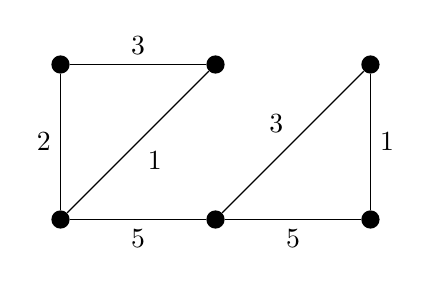
\begin{tikzpicture}[node distance=80]
      \node[fill, scale=0.7, circle]             (a) {};
      \node[fill, scale=0.7, circle, below of=a] (b) {};
      \node[fill, scale=0.7, circle, right of=a] (c) {};
      \node[fill, scale=0.7, circle, right of=b] (d) {};
      \node[fill, scale=0.7, circle, right of=c] (e) {};
      \node[fill, scale=0.7, circle, right of=d] (f) {};
      \tikzset{node distance=10};
      \draw (a) to node[midway, left] {2} (b);
      \draw (b) to node[midway, below right] {1} (c);
      \draw (c) to node[midway, above] {3} (a);
      \draw (b) to node[midway, below] {5} (d);
      \draw (d) to node[midway, above left] {3} (e);
      \draw (d) to node[midway, below] {5} (f);
      \draw (e) to node[midway, right] {1} (f);
     \end{tikzpicture}
    \caption{Graphe non-orienté pondéré}
    \label{fig:graphe-pondere}
  \end{figure}

  \begin{defn}
    Étant donné $G' = (V', E')$, on dit que $G'$ est un \textit{arbre} si $G'$ est connexe et acyclique.
  \end{defn}

  \question{
    Montrer que les trois points suivants sont équivalents :
    \begin{enumerate}
      \item $G' = (V', E')$ est connexe et acyclique ;
      \item $G' = (V', E')$ est connexe et $|E'| = |V'| - 1$ ;
      \item $G' = (V', E')$ est acyclique et $|E'| = |V'| - 1$.
    \end{enumerate}
  }

  \begin{defn}
    On dit que $G' = (V', E')$ est un  \textit{arbre couvrant} d'un graphe $G = (V, E)$ si
    \begin{itemize}
      \item $V = V'$ ;
      \item $E' \subseteq E$ ;
      \item $G'$ est un arbre.
    \end{itemize}
  \end{defn}

  \begin{defn}
    Étant donné $G = (V, E, p)$ un graphe pondéré, le  \textit{poids} d'un sous-graphe $G' = (V', E')$ est \[
    p(G') := \sum_{e \in E'} p(e)
    .\]
  \end{defn}

  Le problème que l'on essaie de résoudre est le suivant :

  \problem[acpm]{pb:acpm}{
    Un graphe pondéré $G = (V, E, p)$ ;
  }{
    Un arbre couvrant $G'$ de poids $p(G')$ minimal.
  }

  Pour résoudre ce problème, on cherche un arbre couvrant, donc la seule donnée qui nous intéresse est $E'$ (car, à la fin, on a $V = V'$).

  L'algorithme utilisé pour résoudre ce problème est l'\textit{algorithme de Kruskal}.
  C'est un algorithme \textit{glouton}.

  \begin{algorithm}[H]
    \centering
    \caption{Algorithme de Kruskal (résolvant \hyperref[pb:acpm]{\textsc{acpm}})}
    \begin{algorithmic}[1]
      \State $E' \gets \emptyset$
      \State On trie $E$ par ordre croissant des poids \label{algo:kruskal:p2}
      \For {$\{x,y\} \in E$ dans l'ordre~\ref{algo:kruskal:p2}}
        \If{$x \mathrel{\centernot -}^\star_{E'} y$}
          \State $E' \gets E \cup \big\{ \{x,y\} \big\}$
        \EndIf
      \EndFor
      \State \Return $G' = (V, E')$
    \end{algorithmic}
    \label{algo:kruskal}
  \end{algorithm}

  Démontrons la correction totale (\textit{i.e.} correction et terminaison) de l'algorithme de Kruskal (algorithme~\ref{algo:kruskal}).

  \question{Montrer la terminaison de l'algorithme~\ref{algo:kruskal}. Quelle est sa complexité ?}

  \question{Montrer que le graphe $G'$ retourné par l'algorithme~\ref{algo:kruskal} est un arbre.}

  Il ne reste qu'à montrer que l'algorithme de Kruskal retourne un arbre de poids minimal, un arbre optimal.
  Pour cela, c'est souvent la même méthode avec les algorithmes glouton : on rapproche l'optimal du résultat donné par l'algorithme glouton.
  Dans la suite, on notera ACPM pour arbre couvrant de poids minimal.

  On se propose de montrer l'invariant suivant :
  \begin{equation}
    \text{il existe un ACPM $T$ tel que $G' \subseteq T$} \label{eq:kruskal-inv}
  \end{equation}

  On note ici $(V, E) \subseteq (V', E')$ lorsque $(V, E)$ est un \textit{sous-graphe} de~$(V', E')$,  \textit{i.e.} lorsque $V \subseteq V'$, $E \subseteq E'$ et $E \subseteq \wp_2(V)$, où $\wp_2(V)$ est l'ensemble des paires ($\neq $ couples) d'éléments de $V$.

  \question{ Prouver l'invariant~(\ref{eq:kruskal-inv}). }

  \question{Conclure quant à la correction totale de l'algorithme~\ref{algo:kruskal}.}

  \question{Donner un ACPM sur le graphe en figure~\ref{fig:graphe-pondere} en utilisant l'algorithme de Kruskal. On détaillera les étapes de l'algorithme.}

  \section{Quelques problèmes $\mathbf{NP}$-complets sur les graphes.}

  On rappelle le problème 
  \problem[$n$-sat]{n-sat}{
    Une formule $\varphi$ sous $n$-FNC
  }{
    La formule $\varphi$ est-elle satisfiable ?
  }

  \question{Pour quelles valeurs de $n$, \hyperref[n-sat]{\textsc{$n$-sat}} est-il $\mathbf{NP}$-complet ?}

  \subsection{Problème~\hyperref[coloration]{\textrm{\textmd{\textsc{$k$-coloration}}}}.}
  \vspace{-1.5\baselineskip}
  {\hfill \tiny\rmfamily\mdseries [ORAUX CCINP MPI 2023]}

  \begin{defn}
    On dit d'un graphe qu'il est \textit{coloriable} si on peut colorier tous les sommets
du graphe tels que deux sommets voisins sont de couleurs différentes. Un graphe est dit \textit{$k$-coloriable}
s’il est coloriable avec $k$ couleurs.
  \end{defn}

  On considère le problème suivant :
  
  \problem[$k$-coloration]{coloration}{
    Un graphe non-orienté $G = (V, E)$
  }{
    Existe-t-il une $k$-coloration de $G$ ?
  }

  On se propose de montrer que \hyperref[coloration]{\textsc{$k$-coloration}} se réduit au problème~\hyperref[n-sat]{\textsc{$k$-sat}}.

  Dans le but de construire cette réduction, on introduit quelques notations.
  Soit $G = (V, E)$ un graphe non-orienté, et $\mathcal{C}$ un ensemble de~$k$ couleurs.
  On crée les variables $p_{v,c}$ pour $v \in V$ et $c \in \mathcal{C}$.

  \question{
    On commence par construire une FNC qui traduit le fait que deux sommets voisins ne peuvent pas être de la même couleur.
    On procèdera ainsi :
    \begin{enumerate}
      \item Pour $u$ et $v$ deux sommets voisins et une couleur $c$, construire une clause qui traduit que $i$ et $j$ ne peuvent pas être de la même couleur $c$.
      \item Créer une $2$-FNC qui traduit que $u$ et $v$ ne peuvent pas être de la même couleur.
      \item Conclure quant au but initial de la question.
    \end{enumerate}
  }

  \question{
    On souhaite traduire le fait qu'un graphe est $k$-coloriable. Pour cela, il est nécessaire que les
sommets voisins ont des couleurs différentes, et que tous les sommets soient coloriés.
    \begin{enumerate}
      \item Traduire cette deuxième condition pour le graphe $G$ sous la forme d'une FNC.
      \item Conclure en construisant une FNC qui traduit qu'un graphe $G$ est $k$-coloriable.
    \end{enumerate}
  }

  \question{
    Montrer que \hyperref[coloration]{\textsc{$k$-coloration}} se réduit au problème~\hyperref[n-sat]{\textsc{$k$-sat}}.
  }

  \question{
    Montrer que \hyperref[coloration]{\textsc{$k$-coloration}} est dans $\mathbf{NP}$.
    Pour quelles valeurs de $k$ le problème \hyperref[coloration]{\textsc{$k$-coloration}} est-il $\mathbf{NP}$-complet ?
  }

  \subsection{Problèmes~\hyperref[clique]{\textrm{\textmd{\textsc{clique}}}} et \hyperref[clique]{\textrm{\textmd{\textsc{stable}}}}.}

  \begin{defn}
    Étant donné un graphe $G = (V, E)$, on dit qu'un sous-ensemble $V' \subseteq V$ est 
    \begin{itemize}
      \item une \textit{clique} si les sommets de $V'$ sont deux-à-deux reliés ;
      \item un \textit{stable} si les sommets de $V'$ sont deux-à-deux non-reliés.
    \end{itemize}

    La \textit{taille} d'une clique ou d'un stable est $|V'|$.
  \end{defn}

  On considère les deux problèmes suivants :
  \problem[clique]{clique}{
    Un graphe $G = (V, E)$ et  $k \in \mathds{N}$
  }{
    Existe-t-il une clique de taille $ \ge k$ ?
  }

  \problem[stable]{stable}{
    Un graphe $G = (V, E)$ et  $k \in \mathds{N}$
  }{
    Existe-t-il un stable de taille $\ge k$ ?
  }

  \question{Montrer que \hyperref[clique]{\textsc{clique}} se réduit polynomialement à \hyperref[stable]{\textsc{stable}}, puis que \hyperref[stable]{\textsc{stable}} se réduit polynomialement à \hyperref[clique]{\textsc{clique}}.}

  On se propose de montrer la $\mathbf{NP}$-complétude du problème \hyperref[clique]{\textsc{clique}} par réduction polynomiale depuis le problème~\hyperref[n-sat]{\textsc{$3$-sat}}.

  Soit $\varphi$ une formule sous forme $3$-CNF. On note $n$ le nombre de clauses de $\varphi$.
  Soient $(\ell_{i,j})_{i \in \llbracket 1,n\rrbracket, j \in \{1,2,3\}}$ les $3n$ littéraux tels que \[
  \varphi = \bigwedge_{i=1}^n (\ell_{i,1} \lor \ell_{i,2} \lor \ell_{i,3})
  .\]

  On construit le graphe $G = (V, E)$ avec :
  \begin{gather*}
    V = \{(i,j)  \mid i \in \llbracket 1,n\rrbracket, j \in \{1,2,3\}\}\\
    E = \Big\{\,\big\{(i_1,j_1),(i_2,j_2)\big\} \;\Big|\; \ell_{i_1,j_1} \neq \lnot\ell_{i_2,j_2} \text{ et } \lnot \ell_{i_1,j_1} \neq \ell_{i_2,j_2} \text{ et } i_1 \neq i_2 \,\Big\} 
  \end{gather*}

  \question{
    Représenter le graphe construit à partir de la formule \[
      (x \lor x \lor y) \land (\lnot x \lor \lnot y \lor \lnot y) \land (\lnot x \lor y \lor y)
    .\]
  }

  \question{
    Montrer que le problème~\hyperref[n-sat]{\textsc{$3$-sat}} se réduit polynomialement au problème~\hyperref[clique]{\textsc{clique}}.
  }
\end{document}
